\documentclass{beamer}

\usepackage[english, ngerman]{babel}	% Englische und deutsche Rechtschreibung
\usepackage[utf8]{inputenc}				% Umlaute-Darstellung unter Linux

\usecolortheme[]{default}

%-------------------- Titelblattinformationen ----------------------------
\title{Qualitätssicherung in einer Scrum basierten Entwicklungsumgebung}
\subtitle{Kurzvortrag}
\author{David Liebemann, Lucas Küntzer, Tobias Meier}
\institute{Fachhochschule Trier}
%--------------------------------------------------------------------------

\begin{document}

\begin{frame}
%------------------------- Titelblatt -------------------------------------
\titlepage
%--------------------------------------------------------------------------
\end{frame}

\begin{frame}
%----------------------- Scrum allgemein ----------------------------------
\frametitle{Scrum - Schritte}
\only<1>{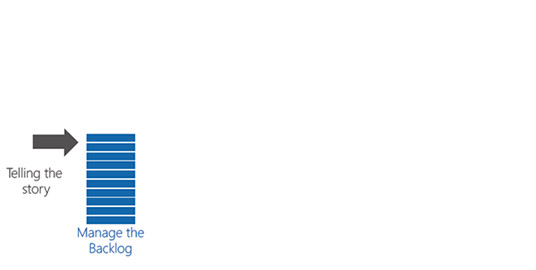
\includegraphics[scale=0.6]{./presGraphics/scrum01}}
\only<2>{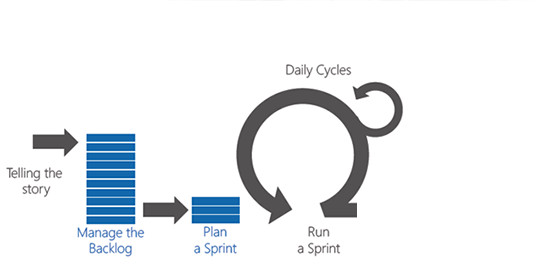
\includegraphics[scale=0.6]{./presGraphics/scrum02}}
\only<3>{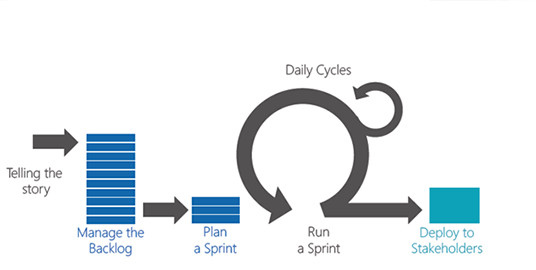
\includegraphics[scale=0.6]{./presGraphics/scrum03}}
\only<4>{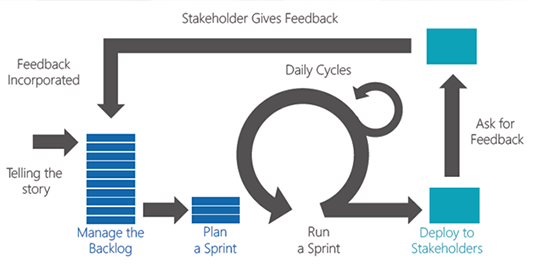
\includegraphics[scale=0.6]{./presGraphics/scrum}}
%--------------------------------------------------------------------------
\end{frame}

\begin{frame}
\frametitle{QA ja, aber wo?}
\begin{block}<1->{nach dem Sprint}
	\invisible<-2>{
		nicht Möglich da: 
		\begin{itemize}
			\item nach einem Sprint ein fertiges Inkrement vorhanden sein soll
		\end{itemize}
	}
\end{block}

\begin{block}<2->{Wärend des Sprintes}
	\invisible<-3>{
		theoretisch Möglich
	}
\end{block}
\only<4>{}	% damit gestoppt wird bevor es zur nächsten Folie geht
\end{frame}

\begin{frame}
\frametitle{Ansprüche an das Qualitätsmanagment}
\begin{itemize}
	\item schnelles Testen
	\begin{itemize}
		\item automatisiert
	\end{itemize}
\end{itemize}
\end{frame}

\begin{frame}
Bild wie Qualitätssicherung in einem Sprint ablaufen könnte
\end{frame}

\end{document}